\chapter{Testdurchführungen}
\label{chap:Testphasen}

Es wurden im Rahmen dieser Arbeit eine grosse Anzahl an Messungen und Testfällen durchgeführt. Die Testkonzepte im digitalen Anhang \ref{AnhangE} geben detailliert Auskunft über die Testdurchführung. Dieses Kapitel beschäftigt sich mit den bedeutendsten Ergebnissen.

\section{Grundlagenmessungen}

Die Grundlagenmessungen geben Auskunft über die Eigenheiten des Sensors. Dabei wurde einerseits  



\subsection{Streuung}

\begin{figure}[H]
	\centering
	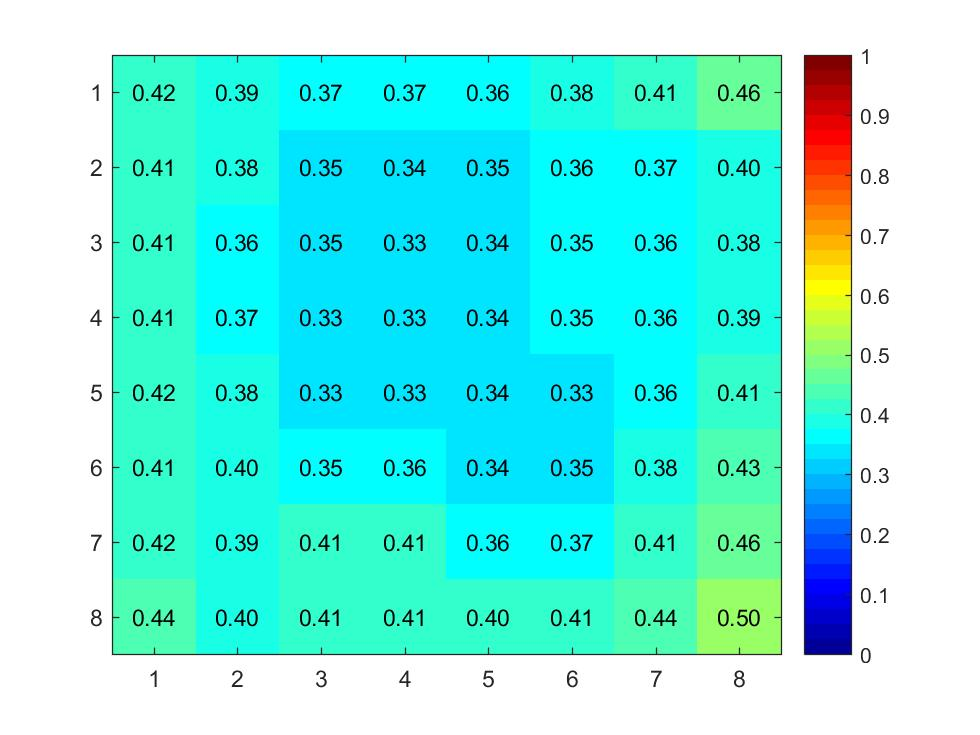
\includegraphics[width=0.5\textwidth]
	{fig/Distanz_140cm_std_.jpg}
	\caption[Streuung der einzelnen Pixel im Vergleich]{Streuung der einzelnen Pixel im Vergleich}
	\label{fig:Streuung}
\end{figure}


\subsection{Reflektion}

\subsection{Streuung}


\subsection{Einfluss Störquellen}

Dieser Abschnitt befasst sich mit den Einfluss von externen Quellen auf den Sensor. Dabei spielen natürliche Einwirkungen wie Luftströme, Umgebungstemperaturen und Lichtquellen einen enormen Einfluss. 



Weitere Störquellen sind Objekte, welche sich innerhalb des \ac{FOV} des Sensors befinden. In Abbildung 26 ist eine



Neben natürlichen Störquellen und Objekten besteht ein enormer Unterschied bei der Bekleidung der zu messenden Personen. 




\section{Personenmessungen}
Bei der Personenmessungen wurden unterschiedliche Probanden in einem Aufzug ausgemessen auf dessen Wärmestrahlung analysiert. 





\begin{figure}[H]
	\centering
	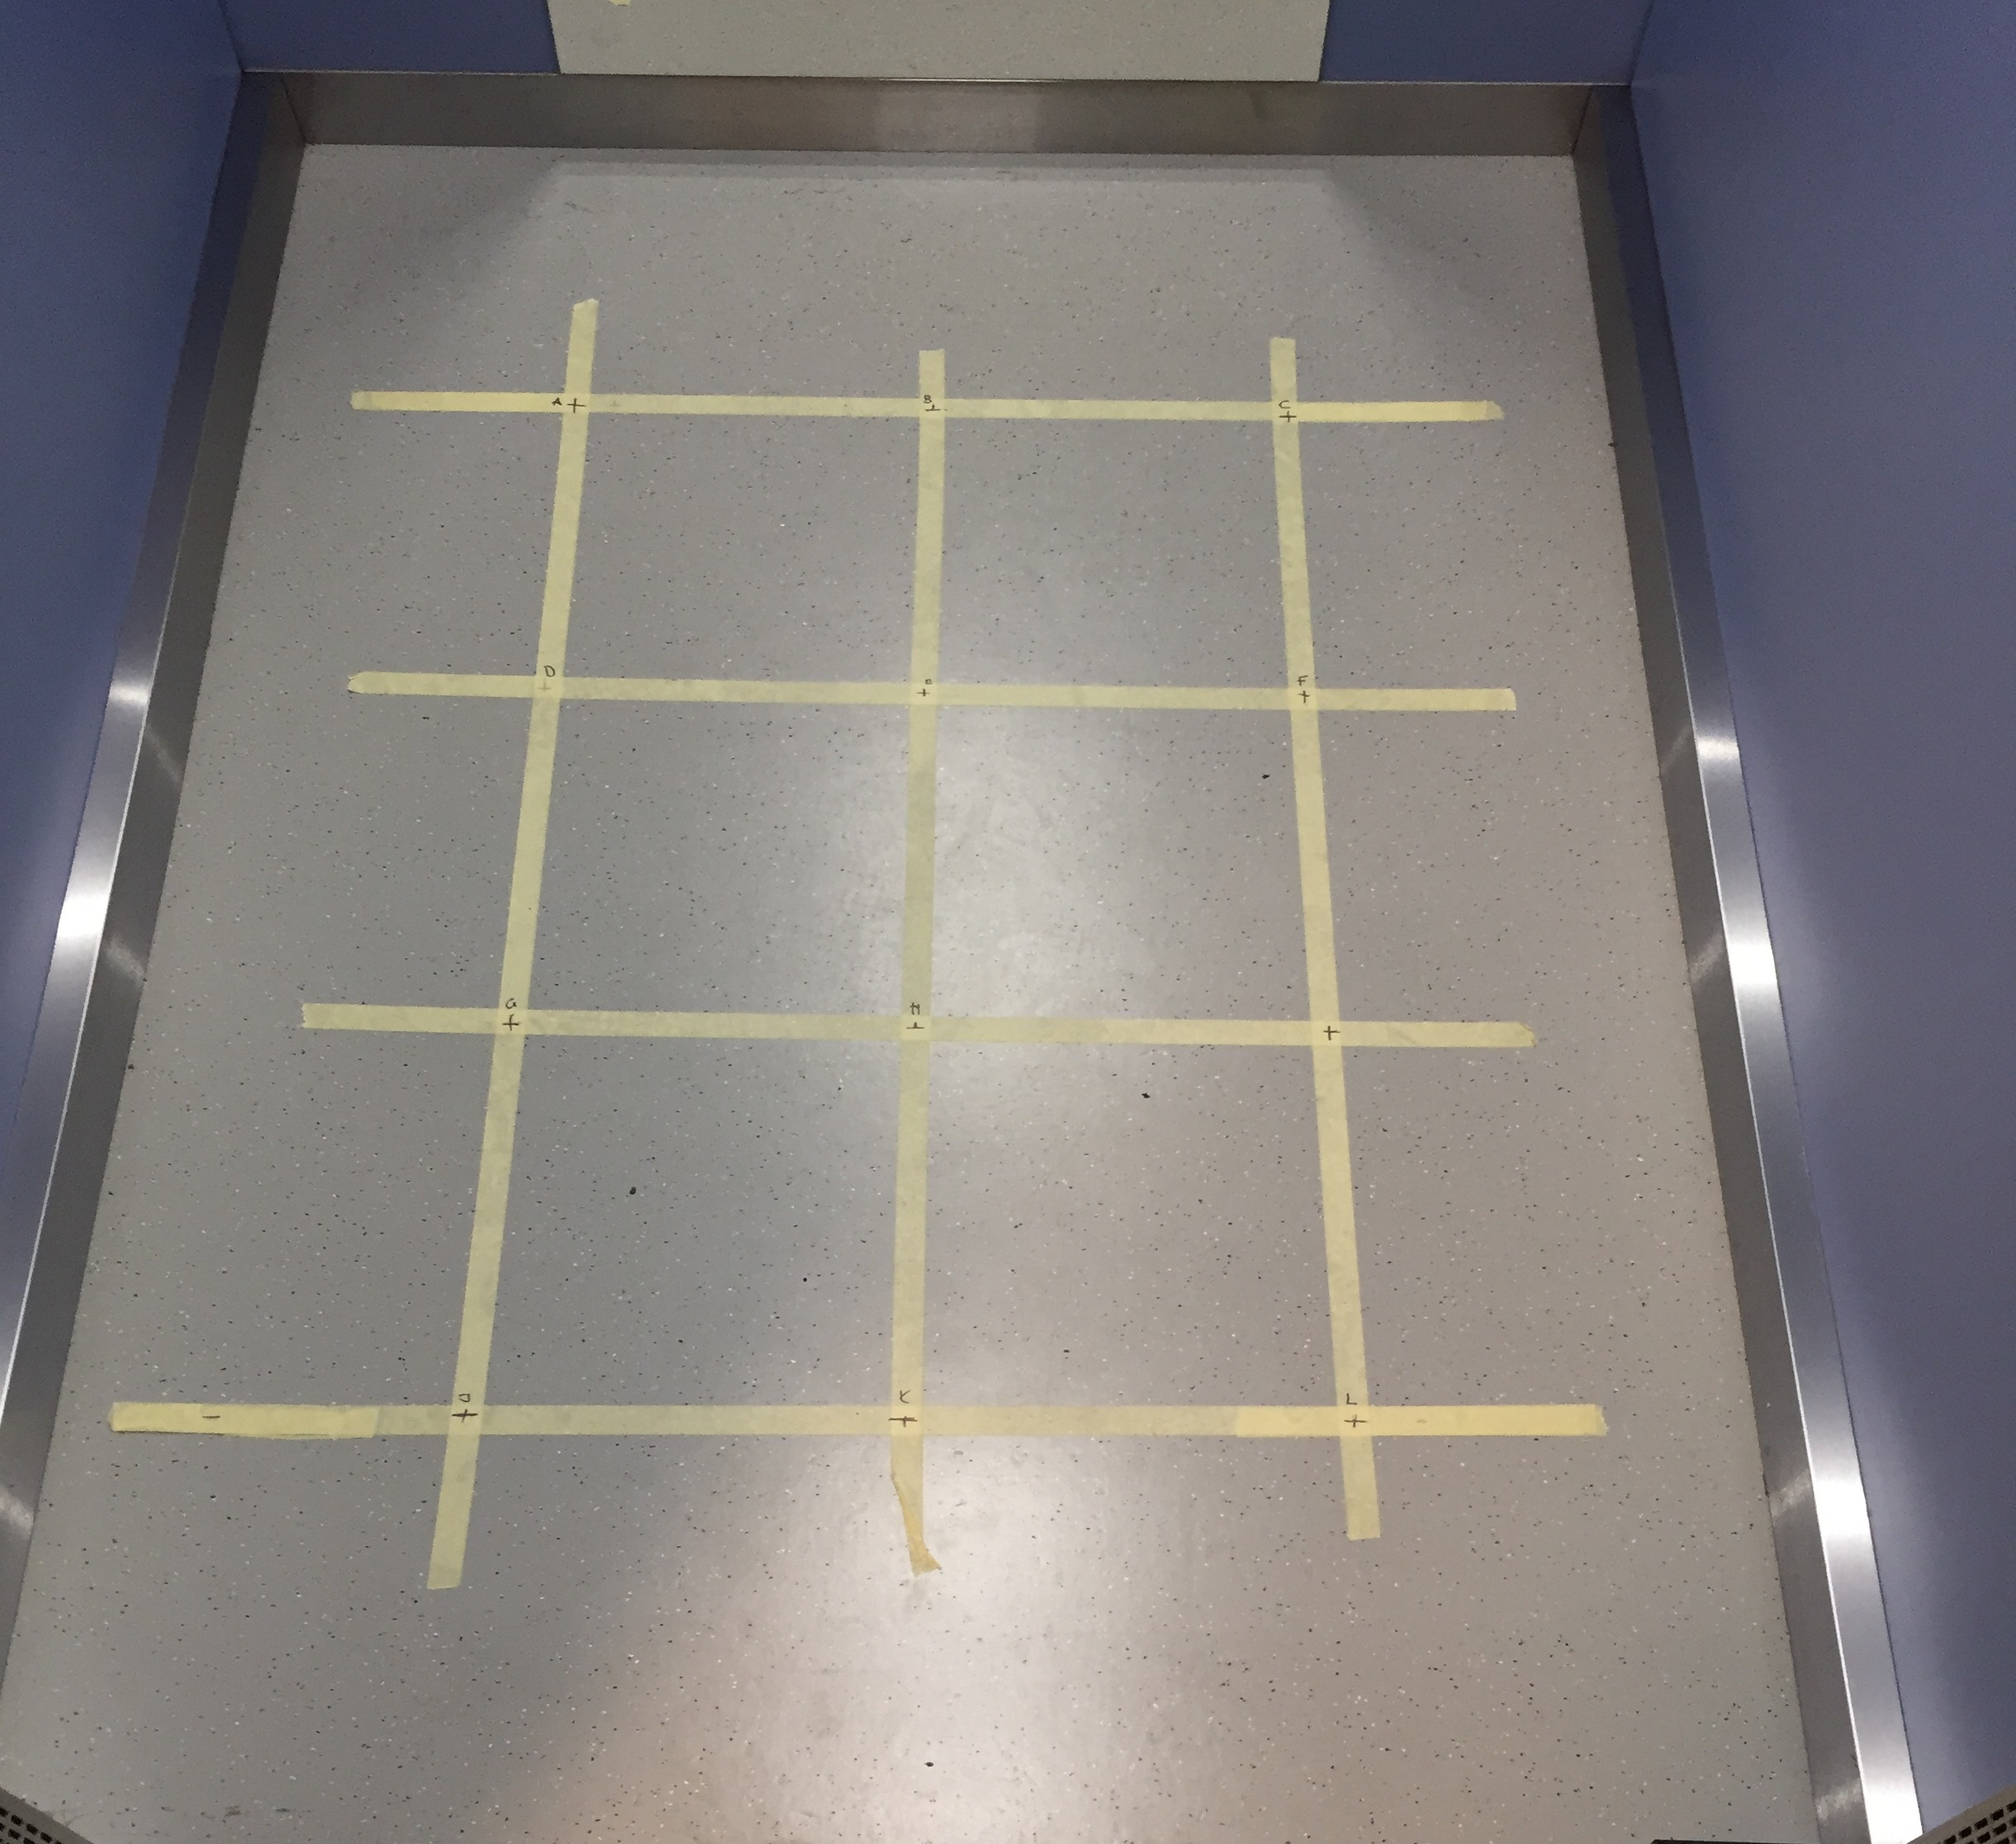
\includegraphics[width=0.8\textwidth, angle=270]
	{fig/Messraster.JPG}
	\caption[Personenmessung Messraster]{Personenmessung Messraster}
	\label{fig:Messraster}
\end{figure}













\section{Fazit}